\documentclass[conference]{IEEEtran}
\IEEEoverridecommandlockouts
% The preceding line is only needed to identify funding in the first footnote. If that is unneeded, please comment it out.
\usepackage{cite}
\usepackage{amsmath,amssymb,amsfonts}
\usepackage{algorithmic}
\usepackage{graphicx}
\usepackage{textcomp}
\usepackage{xcolor}
\usepackage{listings}
\usepackage{breqn}
\usepackage{xcolor}
\usepackage{booktabs}
\def\BibTeX{{\rm B\kern-.05em{\sc i\kern-.025em b}\kern-.08em
    T\kern-.1667em\lower.7ex\hbox{E}\kern-.125emX}}
\lstset{frame=tb,
  language=Python,
  aboveskip=3mm,
  belowskip=3mm,
  showstringspaces=false,
  columns=flexible,
  basicstyle={\small\ttfamily},
  numbers=none,
  numberstyle=\tiny\color{gray},
  keywordstyle=\color{blue},
  commentstyle=\color{dkgreen},
  stringstyle=\color{mauve},
  breaklines=true,
  breakatwhitespace=true,
  tabsize=3
}
\def\BibTeX{{\rm B\kern-.05em{\sc i\kern-.025em b}\kern-.08em
    T\kern-.1667em\lower.7ex\hbox{E}\kern-.125emX}}

\begin{document}

\title{\textbf{Text Summarizer for Amazon Food Reviews}\\}
\author{\textbf{\Large{Yangxiao Bai, Chen-Wei Hung, XiaoZhu Jin, Shi Wen Wong}} \\
South Dakota State University \\
\{bai.yangxiao, chenwei.hung, xiaozhu.jin, shiwen.wong\}@jacks.sdstate.edu \\
}

\maketitle

\begin{abstract}
Online shopping has become a mainstream method of making purchases due to its convenience and efficiency. Reviews play a significant role in assisting shoppers to make purchasing decisions and benefit entrepreneurs by building trust, setting their brand apart from others, and allowing them to make improvements based on the reviews. This project focuses on building a text summarizer for Amazon reviews of fine foods by using Seq2Seq model with an attention mechanism. The goal of this work is to shorten the length of reviews and eliminate irrelevant information while preserving the original context and tone, and ultimately, to save buyers’ time and allow informed purchasing decisions in a timely manner. 
\end{abstract} 

\begin{IEEEkeywords}
Text Summarizer, Seq2Seq, Attention Mechanism, Long-Short Term Memory, Gated Recurrent Unit
\end{IEEEkeywords}

\section{Introduction}
RNN was introduced in 1986 to process sequential data using feedback loops, and it is commonly used for Natural Language Processing related tasks such as language translation, speech recognition, text prediction, and video captioning~\cite{staudemeyer2019understanding}. One drawback RNN experiences is that gradients vanish during backward propagation resulting in the model stopping to learn. In 1997, Long Short-Term Memory (LSTM) was designed by Sepp Hochreiter and J\"{u}rgen Schmidhuber to overcome the gradient-vanishing problem. Furthermore, unlike the traditional RNN, LSTM is capable of learning long-term dependencies effectively through several gates that control what pieces of information should be passed along or discarded. \\ \\
\indent In general, when summarizing a paragraph or a sentence, the meaning of a word is related to the content that precedes and follows it. The Bidirectional RNN works well here, as it can access the inputs from past and future time steps. Additionally, an attention mechanism will be added to the decoding layer to boost the performance of the text summarizer~\cite{vaswani2017attention}. 

\section{Goals and Objectives}
Our goal of this project is to build a neural networks model to summarize any Amazon review on the fine foods product. Our trained model will take in any Amazon fine food review paragraph, and shorten it into a short sentence of summarize. Our review summarizer can help customers to make better decision on purchasing fine food products from Amazon without going through lengthy reviews. Potentially, we can further apply our model to other product categories.\\\\
\indent To load the initial data preparation, we will use the data set from Kaggle - Amazon Fine Food Reviews for our data sets. For our neural network model, we will use Bi-LSTM to perform semantic analysis on our Amazon review training data set. For better learning performance, we will build Seq2seq with Bahdanau Attention to better understand semantic information and output summaries of variable length.
\indent To clean our raw data set, we first selected the \texttt{Summary} and \texttt{Text} columns as $X_S$ and $X_T$ respectively. Then we clean our text by dropping the stopwords \{\texttt{"a", "an", "the", \ldots}\}.

\indent Our text summarizer relies on word embedding. For the word emedding, we need to create a dictionary that cold the number of each vocabulary. The $word_counts$ is the dictionary that holds the number of each vocabulary, $text$ is all the text withing $X_S$ and $X_T$:
\begin{lstlisting}
for sentence in text:
        for word in sentence.split():
            if word not in word_counts:
                word_counts[word] = 1
            else:
                word_counts[word] += 1
\end{lstlisting}

\indent After we created our vocabulary dictionary, we used \emph{Conceptnet Numberbatch's (CN) embeddings} to create a set or embedding weight $We$ for each word $W$:
\begin{equation}
    We = \sum_{i = 1}^{N} We_i
\end{equation}
\indent Lastly, we convert our text, $X_S$ and $X_T$ to integers $It$ with $word_count$ dictionary and the words $W$ that each word has its own embedded weight. $w()$ represent the function to extract the weight of each word.
\begin{equation}
    It_k = \sum_{k = 1}^{N}W_k \in W_S + W_k \in W_T
\end{equation}
\section{Related Work and Preliminary Results}
\subsection{RNN}
RNN is a network model that uses at least one feedback connection to build a sequenced learning process. The model can pass a sequential data stream as input, and for each learning state of single input, it can get experience feedback from the previous learning state to improve the current learning accuracy. The Bidirectional RNN added a backward learning sequence to the RNN model so that the model can perform machine learning forward and backward to two separate recurrent nets~\cite{vu2016bi} ~\cite{schuster1997bidirectional}. The RNN provided mechanics to remember the historical information for each learning stage from its previous training, which is very helpful for the time series predictors. Nallapati et al ~\cite{nallapati2016Aug} implemented an abstractive text summarization model using RNN. They used a bidirectional GRU-RNN as the encoder and a uni-directional GRU-RNN as the decoder with attention mechanisms to optimize the encoder and decoder. In recent research, traditional RNN has rarely been used due to its limitation: If the learning process is very long, the RNN will have a significant gradient vanishing problem which loses weight from the previous learning stage to update the current network. Many techniques such as GRU (Gated Recurrent Unit) and LSTM (Long-Short Term Memory) are implemented to solve the RNN’s gradient vanishing problem. Both techniques added a logic gate called forget gate and a memory cell to RNN neurons. The forget gate filters the necessary information, and the memory cell stores those experiences throughout the training. The project will use LSTM-RNN as the machine-learning model to train the text summarizer.
\subsection{LSTM}
LSTM is an improvement of RNN to solve its’ gradient vanishing problem. In a long-term learning process of RNN, the feedback for each state will gradually lose weight as learning continues and finally have no influence. This will make the final trained model work properly only when the input data is similar to the late parts of the training data. Therefore, for each RNN neuron, only a specific range of feedback can help the learning process, which limits the size of the input data. The LSTM model stores all necessary feedback filtered from all previous learning states by using logic gates that can memorize and forget ~\cite{hochreiter1997long} ~\cite{gers2000learning}. Each LSTM RNN neuron has a memory block that contains a memory cell and three gates: forget gate, input gate, and output gate. The memory cell stores the experience learned from previous stages. The forget gate decides which information can access the memory cell, the input gate updates the information in the memory cell, and the output gate decides what new information can be sent to the next stage. Based on LSTM and RNN, there are many variant machine learning models were implemented such as BDLSTMs (Bidirectional Long-Short Term Memory) and Seq2Seq LSTM-RNN. Munzir et al ~\cite{Munzir2019} implemented and compared text summarization models using GRU-RNN and LSTM for analyzing Bengali text and found that the text summarization model with LSTM has around 23\% higher accuracy than the text summarization model using GRU-RNN. For their LSTM model, they put sentences as sequences of words and put each sequence into the model which contains an embedding layer, an LSTM layer, and a Dense layer. The embedding layer converts sequences of words into vectorized data, and the LSTM layer process the vectorized data and sends the results to the next dense layer. 
\subsection{Text summarizer}
A text Summarizer is a tool to summarize long sentences or paragraphs by finding the subsets of data that can represent the information of the whole text set and present it in a conci annotationse manner to focus on the most important parts of the text ~\cite{sinha2018extractive}. The text summarizer has two different types of approaches including attractive and extractive text summarization ~\cite{pai2014}. The abstractive text summarization read through the sentence and generates meaningful summaries. It is always trained by using Supervised machine learning models. The extractive text summarization combines the extracted information as the summary without knowing the major meaning of the sentence. It always uses unsupervised machine learning techniques as the trainer. This project will focus on the implementation of an abstractive text summarizer.
\subsection{Seq2Seq}
Seq2Seq (Sequence-to-sequence) is a machine learning technique used to handle situations like natural language processing when both input and output are sequences. It creates 2 hidden layers called the encoder and decoder in the network. The encoder processes the data into a machine-learning model to transform it into a fixed-length vector representation, which will be used as the initial hidden state of the decoder which uses another machine-learning model to generate the output ~\cite{sutskever2014sequence} ~\cite{vinyals2015show}. This technique has been widely used to build text summarizers. Masum et al ~\cite{Masum2019} built an abstractive text summarizer by using a 2-layer Bidirectional RNN with LSTM as the encoder and an Attention model as the decoder to generate the short summary. This project will use Bidirectional RNN with LSTM as the encoder layer and RNN with LSTM as the decoder layer. To improve the efficiency of extracting necessary information, the optimization method called Attention will be added to the decoder layer to make it focus on the selective sequence of input data instead of the whole context.
\subsection{Bahdanau Attention}
The Attention is one of the optimizations to Seq2Seq machine learning by making the decoder only look at the selected part from the encoder’s output. By using the Attention model, the machine can focus on the meaningful context without looking at the whole text, which can make the training and summarization more efficient. The machine’s Attention model can be trained by using gradient descent. There are many Attention models implemented such as Addictive Attention or Bahdanau Attention. The concept of Bahdanau Attention was originally proposed by Dzmitry et al ~\cite{bahdanau2014neural}. It calculates the alignment scores for the encoder’s output and stores them as a vector and processes it with the Softmax. The decoder will use these scores in the vector as weights to decide the contents to focus on and ignore. With the introduction of the RNNsearch(attention mechanism) into the decoder, the performance of machine translation has been greatly improved. Regardless of the sentence length, it is much more robust than the length of a source sentence. This technology is also good for improving the performance of text summarization. Bahdanau attention often cooperates with LSTM RNN and Seq2Seq to generate a text summarizer. Masum et al ~\cite{Masum2019} used the Bahdanau attention model to build the decoder to cooperate with the encoder implemented with Bidirectional RNN and LSTM and had only a few wrong outputs. This project will add Bahdanau Attention to the Seq2Seq model to help the machine extract meaningful information from redundant comments to improve the machine’s overall efficiency.
\section{Methodology}
\begin{figure}[h]
\centering
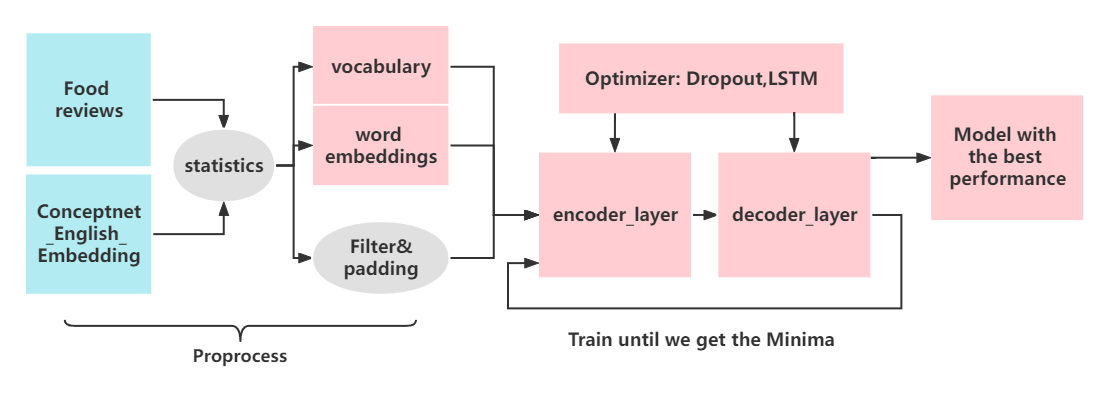
\includegraphics[width=0.5\textwidth]{imgs/System_Structure.png}
\caption{System structure}
\label{fig:System_Structure}
\end{figure}
\begin{flushleft} 
We implemented the following steps using PyTorch.
\end{flushleft}
\subsection{Data Preparation}
This dataset consists of more than 50,000 Amazon reviews of fine foods posted over a 10-year period from October 1999 to October 2012. It contains information about the product ID, user ID, profile name, helpfulness numerator, helpfulness denominator, review score, time, summary, and text. Here, “text” represents reviews that customers provided; for ease of understanding, we rename “text” to “reviews.” \\
\indent Before cleaning the data, we load the dataset using pandas. For this project, we focus only on the summary and review columns, so the other columns are being dropped, and null values are being removed. We then replace contractions with their full/longer forms using the list posted on~\cite{unknown1}. We also convert every word of the summaries and reviews to lowercase and remove any unwanted characters, such as the dash, hyphen, and @. We import the Natural Language Toolkit (NLTK), which includes a list of 40 stop words, into our model. We only remove stop words from the reviews because they are not too important to the training process. By doing so, the size of the dataset is reduced, which speeds up the training process. After cleaning the summaries and reviews, we use ConceptNet Numberbatch (CN) to map words to word embeddings. If certain words do not exist in CN, we assign the words to UNK tokens. Before sorting the reviews and summaries by length from shortest to longest, we add a GO token and an EOS token at the front and end of each sentence respectively. To obtain more meaningful data, if the UNK tokens appear more than once in the reviews or more than 0 times in the summaries, the reviews and summaries are being removed. At this point, we are ready to build a model.


\subsection{Build a Model}
\indent We used a seq2seq model with an encoder and decoder architecture. We want to train the model in batches, so we defined a function to create mini batches. Additionally, we padded zeros at the end of the sentence after the EOS token to ensure that the lengths are the same if sentences are shorter than the maximum length of a sentence within a mini batch. After these, the batch size was kept at 64. \\

\indent The encoder takes in vocab size, hidden size, and dropout rate as parameters. It takes the entire input sequence word by word for each sentence in a batch and then generates a sequence of outputs and hidden states using the Gated Recurrent Unit (GRU). The GRU is also known as a method to solve the vanishing gradient problem of RNN. It consists of an update gate and a reset gate, which helps the model determine how much past information it should pass along or forget. The hidden state takes information from the previous time steps’ outputs, inputs, and hidden states at each time step. Then, when we reach the last hidden state, it still contains vital information from before. The encoder will return a sequence of outputs for each sentence and the last hidden state. The last hidden state is also called the context vector. \\
\indent The decoder also takes in the vocab size, hidden size, and dropout rate as parameters. The hidden size and dropout rate for the encoder and decoder are the same, which are 100 and 0.2, respectively. The context vector from the encoder which contains the encoder’s last hidden state and the previous decoder’s output is the input for the decoder. The decoder produces the predicted summary word by word, and it will start after the GO token and stop when it reaches the EOS token. The decoder also returns all the hidden states for each sequence. \\
\indent To optimize the model, we implemented the attention mechanism into the decoder. The attention mechanism can make the decoder focus on the selected info from the encoder’s output. Instead of using the last hidden state from the encoder, the attention decoder uses the encoder’s output and all of its hidden states to generate input with the previous decoder’s output. The attention decoder first, calculates the alignment score, then, SoftMax the alignment score and multiplies the result with the encoder’s output to get the context vector, then, concatenates the context vector with the previous decoder’s output to pass into the decoder as the input. Based on the methods to calculate, we made two different attention variants. \\
\indent The first implemented attention mechanism was the Bahdanau attention. It calculates the alignment score by adding the decoder’s previous hidden state and the encoder’s hidden states, putting the sum into a Hyperbolic Tangent function as alignment weights (\ref{ba1}), multiplying it with a trainable vector, and SoftMax the result (\ref{ba2}).
\begin{dmath}
    \label{ba1}  
\text{Alignment Weights} = tanh(W_{Decoder} \cdot H_{Decoder} + W_{Encoder} \cdot H_{Encoder})
\end{dmath} 
 Then, the decoder multiplies the alignment score with the encoder’s output to generate the context vector (\ref{ba3}), concatenates the context vector with the previous decoder’s hidden state, and feeds them into the decoder as input.

\begin{equation}
    \label{ba3}
\text{Context Vector} = \text{Encoder Output} \cdot \text{Alignment Score}
\end{equation}  
\\
\indent The second implemented attention mechanism was the Luong attention. This mechanism was developed from Bahdanau attention. It calculates the alignment score by using the current decoder’s hidden state instead of the previous decoder’s hidden state. Therefore, the attention is introduced after getting the current decoder’s hidden state by using the previous decoder’s hidden state and the encoder’s output. The Luong attention first, calculates the alignment score by multiplying the current decoder’s hidden state with the encoder’s hidden states (\ref{la1}),
\begin{equation}
    \label{la1}
    \text{Alignment Score} = \mathrm{H}_{encoder}^{} \cdot \mathrm{H}_{decoder}^{}
\end{equation}  
then multiplies the encoder's output with softmaxed alignment score to generate the context vector (\ref{la2}), concatenates it with the current decoder’s hidden state, and passes them into the next decoder.
\begin{equation}
    \label{la2}
    \text{Context Vector} = \mathrm{Output}_{\text{Encoder}}^{} \cdot softmax(\text{Alignment Score})
\end{equation}  
\\
\indent For the final part, we build the seq2seq model. It takes in an encoder and attention decoder. It will produce a final prediction for each batch, and we use that prediction to compute the loss when starting training. 



\indent The second implemented attention mechanism was the Luong attention. This mechanism was developed from Bahdanau attention. It calculates the alignment score by using the current decoder’s hidden state instead of the previous decoder’s hidden state. Therefore, the attention is introduced after getting the current decoder’s hidden state by using the previous decoder’s hidden state and the encoder’s output. The Luong attention first, calculates the alignment score by multiplying the current decoder’s hidden state with the encoder’s hidden states (\ref{la1}),
\begin{equation}
    \label{la1}
    \text{Alignment Score} = \mathrm{H}_{encoder}^{} \cdot \mathrm{H}_{decoder}^{}
\end{equation}  
then multiplies the encoder's output with softmaxed alignment score to generate the context vector (\ref{la2}), concatenates it with the current decoder’s hidden state, and passes them into the next decoder.
\begin{equation}
    \label{la2}
    \text{Context Vector} = \mathrm{Output}_{\text{Encoder}}^{} \cdot softmax(\text{Alignment Score})
\end{equation}  
\\
\indent For the final part, we build the seq2seq model. It takes in an encoder and attention decoder. It will produce a final prediction for each batch, and we use that prediction to compute the loss when starting training. 



\subsection{Train and Evaluate the Model}
Instead of training an entire dataset, which could be time consuming, we used a subset between 20,000 to 25,000. We trained median sequence lengths, and randomly split the dataset into training and validation sets, and there is no overlap between the two datasets. The training set was used only for training purposes, and the validation set was used for detecting whether the model underfit or overfit. To prevent gradient explosion, which occurs when large error gradients accumulate, resulting in extremely large updates to weights during training, we applied gradient clipping by norm (\ref{eqn1}). By selecting a specific value as threshold, if the gradient gets too large, it will be clipped to keep it less than the threshold. More specifically, in this project, it rescales gradients so that their norm will not exceed the threshold of 5 (we choose this value).
\begin{equation}
    \label{eqn1}
    if \left\| g \right\| \ge v \text{ then } g \gets \frac{g}{\left\| g \right\|}*v
\end{equation}    
where v is the threshold. \\

For the optimizer, we used Adam to update weights more efficiently with a default learning rate of 0.001.
The Adam optimizer is a combination of Momentum (\ref{eqn2}) and Root Mean Square Propagation (\ref{eqn3}) where $m_t$ and $m_t-1$ are aggregates of gradients at time t and t - 1, $v_t$ and $v_t-1$ are sum of square of past gradient at time t and t - 1, $\beta$ is moving average parameter, $\delta L$ is derivative of Loss function, $\delta L$ is derivative of weights at time t. It iteratively computes the bias-corrected estimates from those two gradient descent methods and uses these results to update the moving average parameters.
\begin{equation}
    \label{eqn2}
    \mathrm{m}_{t}^{} = \beta\mathrm{m}_{t-1}^{} + (1-\beta)\left[ \frac{\delta L}{\delta \mathrm{w}_{t}^{}} \right]
\end{equation}    
\begin{equation}
    \label{eqn3}
    \mathrm{v}_{t}^{} = \beta\mathrm{v}_{t-1}^{} + (1-\beta)\left[ \frac{\delta L}{\delta \mathrm{w}_{t}^{}} \right]^2
\end{equation}    
 Additionally, Cross Entropy (\ref{eqn4}) was used to evaluate the performance of the model. 
\begin{equation}
    \label{eqn4}
    L = - \dfrac{1}{N} \sum_{i = 1}^{N} y_i * log(p_i)
\end{equation}    
where $y_i$ is the target and $p_i$ is the prediction. We only computed the loss using the non-zero elements on the target and prediction so we removed the padded zeros from them. 

For now, we set the number of epochs to 20, so the model will stop after running the entire training dataset 20 times.  \\ \\ 
\indent Moving forward, we will implement early stopping, which would stop the model if loss is not decreasing anymore and also prevent overfitting. Furthermore, we plan to create a profanity filter, apply an attention mechanism with LSTM to boost the accuracy of the model, and plot a graph to show the training and validation error.


\subsection{Calculation of LSTM}
\indent GRU and LSTM are known as solutions to the vanishing gradient problem of RNN. GRU consists of an update gate, $z_t$, and a reset gate, $r_t$, which helps the model determine how much past information it should pass along or forget. The hidden state takes information from the previous time steps’ outputs, inputs, and hidden states at each time step. Then, when we reach the last hidden state, it still contains vital information from before. The encoder will return a sequence of outputs for each sentence and the last hidden state. The last hidden state is also called the context vector. The following is how hidden states, $h_t$, in GRU are calculated: 
\begin{align}
z_t &= \sigma(W_z \cdot [h_{t-1},x_t]) \\
r_t &= \sigma(W_r \cdot [h_{t-1},x_t]) \\
\Tilde{h}_t &= tanh(W\cdot [r_t*h_{t-1},x_t]) \\
h_t &=(1-z_t)*h_{t-1}+z_t*\Tilde{h}_t 
\end{align}
where $W_z, W_r, W$ are trainable parameters. \\
\indent LSTM consists of a forget gate, $f_t$, an input gate, $i_t$, and an output gate, $o_t$. The context vector is the last cell state, $c_t$, and the last hidden state, $h_t$. The formulas to compute the cell state and hidden state are as follows:
\begin{align}
f_t &=\sigma(W_f\cdot [h_{t-1},x_t] +b_f) \\
i_t &=\sigma(W_i\cdot [h_{t-1},x_t] +b_i) \\
o_t &=\sigma(W_o\cdot [h_{t-1},x_t] +b_o) \\
\Tilde{c}_t &= tanh(W_c \cdot [h_{t-1},x_t] +b_c) \\
c_t &= f_t \cdot c_{t-1} + i_t*\Tilde{c}_t \\
h_t &= o_t \cdot tanh(c_t) 
\end{align}
where $W_f, W_i, W_o, W_c, b_f, b_i, b_o, b_c$ are trainable parameters.
\indent The encoder takes in vocab size, hidden size, and dropout rate as parameters. It takes the entire input sequence word by word for each sentence in a batch and then generates a sequence of outputs and a context vector. \\
\indent The decoder also takes in the vocab size, hidden size, and dropout rate as parameters. The hidden size and dropout rate for the encoder and decoder are the same, which are 100 and 0.2, respectively. The context vector from the encoder is the input for the decoder. For GRU, the context vector is the last hidden state, while for LSTM, the context vector is the last cell state and hidden state. \\
\indent After training, the decoder produces the predicted summary word by word, and it will start after the GO token and stop when it reaches the EOS token. The input sequence first gets pass to the encoder to get a context vector. Then, we initialize the decoder with the context vector of the encoder and pass the GO token as an input to the decoder. After a time step, the output of the decoder is the probability of the next word and then the word with the highest probability will be selected. We then proceed to pass the word as an input in the next time step and update the hidden state and cell state (if we are using LSTM). We repeat this process until we reach the END token. The output of the decoder is the summary. \\
\indent To optimize the model, we implemented the attention mechanism into the decoder. The attention mechanism can make the decoder focus on the selected info from the encoder’s output. Instead of using the last hidden state from the encoder, the attention decoder uses the encoder’s output and all of its hidden states to generate input with the previous decoder’s output. The attention decoder first, calculates the alignment score, then, SoftMax the alignment score and multiplies the result with the encoder’s output to get the context vector, then, concatenates the context vector with the previous decoder’s output to pass into the decoder as the input. Based on the methods to calculate, we made two different attention variants. \\
\indent The first implemented attention mechanism was the Bahdanau attention. It calculates the alignment score by adding the decoder’s previous hidden state and the encoder’s hidden states, putting the sum into a Hyperbolic Tangent function as alignment weights (\ref{ba1}), multiplying it with a trainable vector, and SoftMax the result (\ref{ba2}).
\begin{dmath}
    \label{ba1}
    \text{Alignment Weights} = tanh(W_{Decoder} \cdot H_{Decoder} + W_{Encoder} \cdot H_{Encoder})
\end{dmath}  

\begin{equation}
    \label{ba2}
\text{Alignment Score} = Softmax(\mathrm{V}_{}^{T} \cdot \text{Alignment Weights})
\end{equation} 

For now, we set the number of epochs to 20, so the model will stop after running the entire training dataset 20 times.  \\ 


\section{Evaluation Plan}
\subsection{Real datasets}
The dataset we use is Amazon Fine Food Reviews which contains more than 500000 records, spanning a period of more than 10 years. This dataset also provides summaries labeled by humans so that we can train our model to learn this ability to generalize. 
\subsection{Evaluation Measurement}
we will use both metric-based and human-subject evaluations to evaluate our model. Since we get the original summaries in the datasets, we can subjectively judge whether machine-generated generalization results outperform humans.  Besides, the performance of various text summarization methods is reported on shared DUC datasets using an automatic evaluation framework, ROUGE~\cite{lin-2004-rouge},which is DUC’s official evaluation metric for text summarization. Our experiments are based on the calculation of ROUGE sore in mutiple dataset.

\begin{figure}[h]
\centering
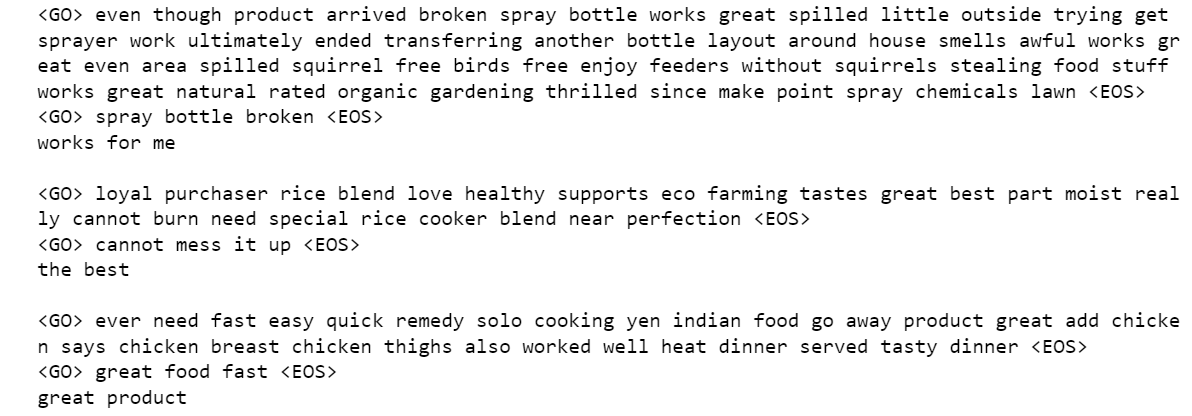
\includegraphics[width=0.5\textwidth]{imgs/Results.png}
\caption{summarization results}
\label{fig:Results}
\end{figure}
The ROUGE score has many metrics, The ROUGE-1, ROUGE-2, ROUGE-l are the most widely used. ROUGE-1 Precision and Recall compare the similarity of uni-grams between reference and candidate summaries.ROUGE-2 Precision and Recall compare the similarity of bi-grams between reference and candidate summaries. By bi-grams, we mean each token of comparison is 2 consecutive words from the reference and candidate summaries. ROUGE-L Precision and Recall measures the Longest Common Subsequence (LCS) words between reference and candidate summaries. By LCS, we refer to word tokens that are in sequence, but not necessarily consecutive. \\
Figure\ref{fig:Results} shows the results of our model on the Amazon review datasets. We apply rouge evaluation framework on it. First, we import python package ROUGE to our project, then convert the result format. The framework will get the average of scores for each pair of sentence. In this way, we get to do quantitative analysis of the performance of text summarization models.\\
\subsection{Comparative Experiment}
\begin{table}
\centering
\caption{\label{tab:Results}Rouge scores for each method}
\begin{tabular}{llll} 
\toprule
\textbf{Method}                              & \textbf{Rouge-1~} & \textbf{Rouge-2} & \textbf{Rouge-l}  \\
\textbf{GRU(baseline)}                       & 0.189             & 0.074            & 0.187             \\
\textbf{LSTM+Pre-train}          & 0.109             & 0.012            & 0.106             \\
\textbf{Bahdanau Attention+Pre-train} & 0.232             & 0.122            & 0.231             \\
\textbf{Luong Attention+Pre-train}    & \textbf{0.276}    & \textbf{0.159}   & \textbf{0.274}    \\
\bottomrule
\end{tabular}
\end{table}
We design comparative experiment on 4 different methods, and record the averge ROUGE score on the test dataset. The consequence is listed in Table~\ref{tab:Results}. Experiment result shows the method GRU+Luong Attention+Pre-trained embedding achieve the best performance with the highest F1 score 0.274. Although the score is not high, it shows that this model has the ability to supplement the key information of the text. 
\subsection{conclusion}
This paper presents a RNN-based model for abstractive summarization tasks. We implement the Seq2seq structure with attention via network model in pytorch. The proposed model is able to output summaries sequence of indeterminate length. We design comparative experiment and the result suggest that GRU+Luong Attention+Pre-trained embedding is our proposed method on this Food review summarization task. 

\bibliographystyle{IEEEtran}
\bibliography{references.bib}
\end{document}
